\chapter{Low Energy Lattice Dynamics}\label{ch:lowen}
In this chapter we investigate the lattice dynamics of La$_{1.94}$Sr$_{0.06}$CuO$_{4+\delta}$ as observed by neutron scattering with the intention of comparing with simulations performed in chapter \ref{ch:simulation}. Similar to the elastic reciprocal space maps done with the FlatCone analyser in the previous chapter, we now look at the same maps with finite energy transfers. These are compared to experiment by constructing neutron-weighted band structures and 2D $(Q_x,Q_y$ maps from simulation data. In addition, 

We also look at soft phonons related to the LTO-LTT transition in La$_2$CuO$_{4+\delta}$. These phonons have shown interesting behavior in LSCO, and we are interested in how this picture changes when working with oxygen-doped samples. Finally, we look at the superstructures discussed in the previous chapter and search for possibly related dynamics.

\section{Acoustic Phonons and Simulation Validation}
We start by considering measurements performed on IN8 at ILL, using the FlatCone secondary spectrometer as described in section \ref{sec:single_crystal_superstructures}. By measuring a large region of $\bm{Q}$ while changing the energy transfer $\hbar\omega$, we can build up a three-dimensional data-set of low energy phonon dispersions. The sample is a single crystal La$_{1.94}$Sr$_{0.06}$CuO$_{4+\delta}$ ($T_\text{c} = \SI{37.5}{\kelvin}$) aligned in the $a$-$b$ plane. The elastic signal was shown in the previous chapter, figure \ref{fig:lscoo_ab_elastic}. The spectroscopic measurements were performed from \SIrange{1}{16}{\milli\eV} in steps of \SI{1}{\milli\eV}.

\begin{figure}
    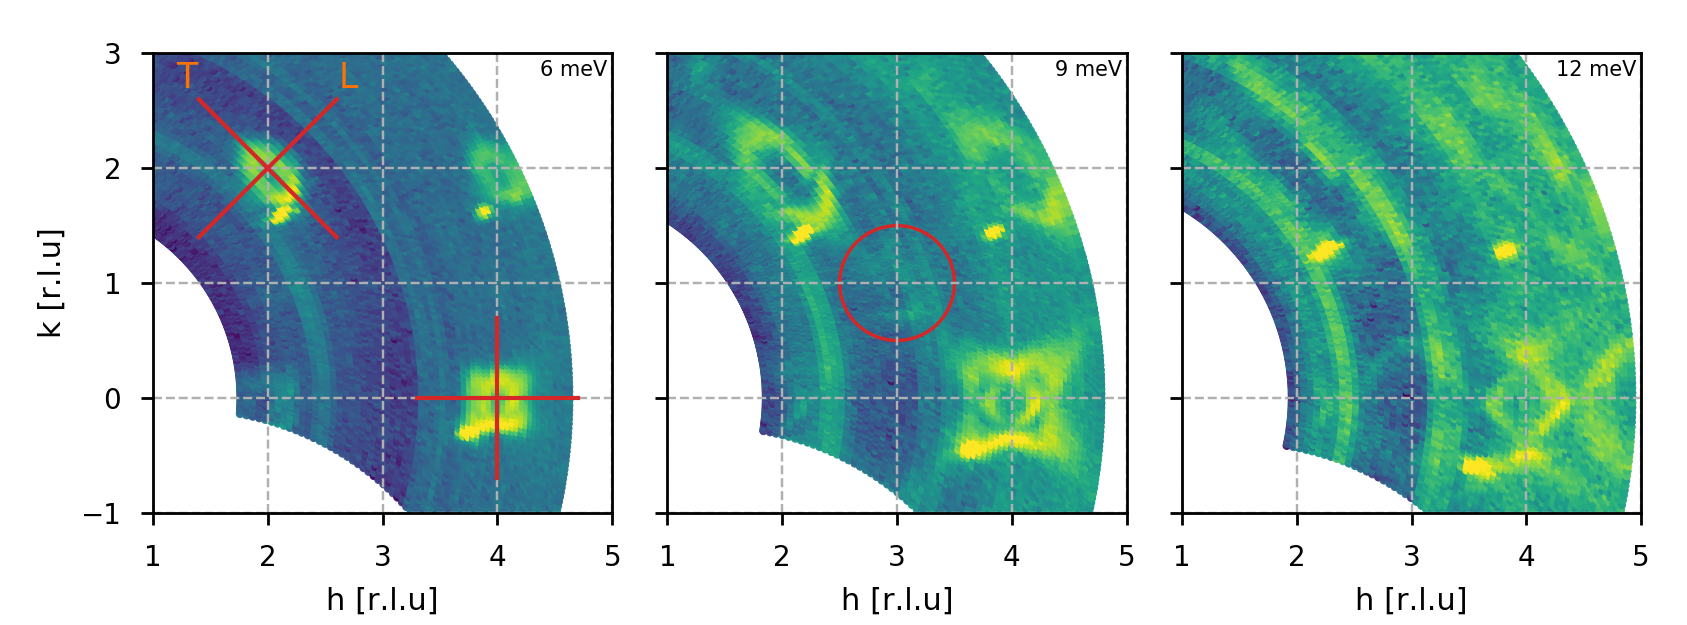
\includegraphics[width=\textwidth]{fig/lowen/flatcone_colorplots.png}
    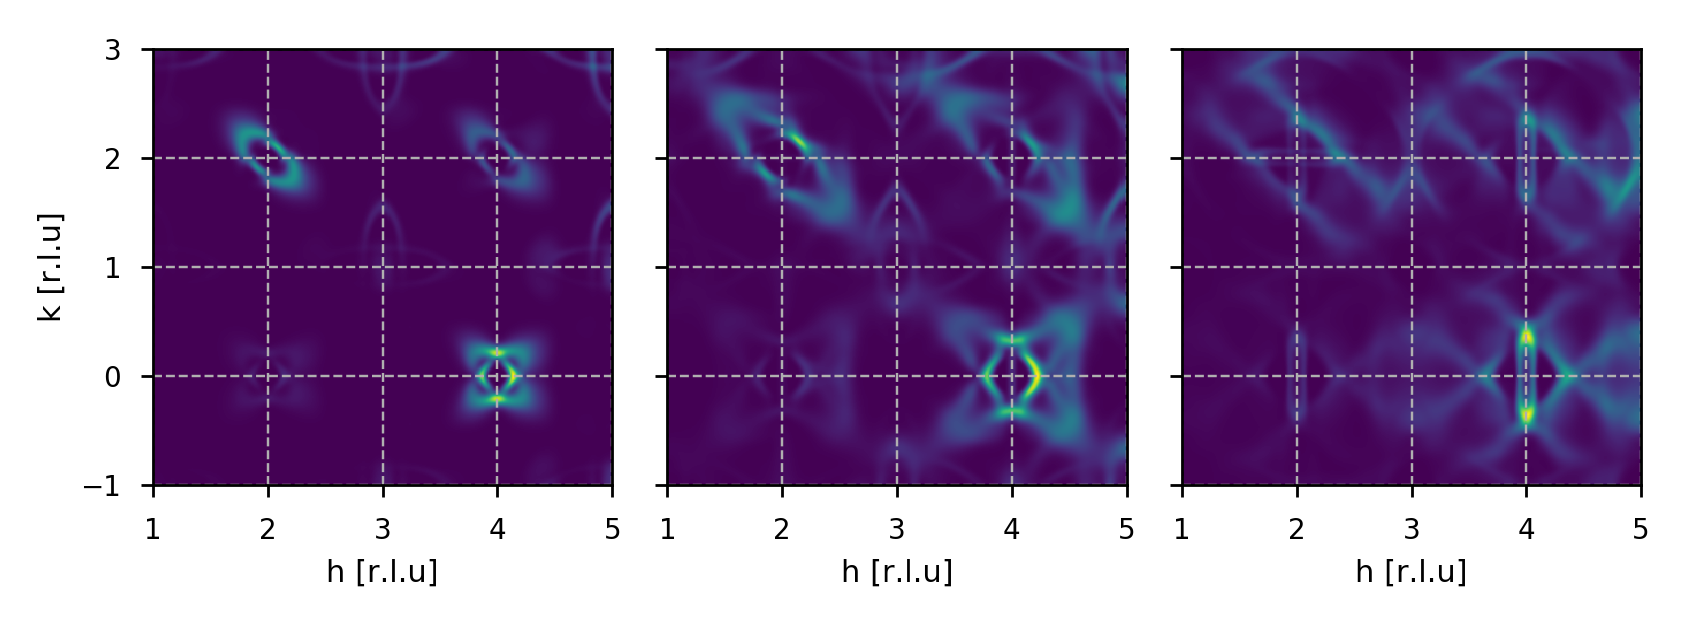
\includegraphics[width=\textwidth]{fig/lowen/simulation_colorplots.png}
    \caption[Flatcone raw inelastic]{FlatCone data of La$_2$CuO$_{4+\delta}$ in the $a$-$b$ at three energies and simulation data of La$_2$CuO$_{4}$ at the same energies. \textbf{Top}: Raw data at \SIlist{6;9;12}{\milli\eV} annotated with cut directions in the leftmost figure. In addition, the middle figure highlights a small amount of spectral weight observed in a narrow range of energies near (310). \textbf{Bottom}: Simulation data at energies corresponding to the top row. Details about the simulation data is given in the text.}
    \label{fig:flatcone_raw_inelastic}
\end{figure}

Figure \ref{fig:flatcone_raw_inelastic} shows representative data at \SIlist{3;9;12}{\milli\eV} in the top row. The bottom row shows simulations results of La$_2$CuO$_4$ in the Low-Temperature Orthorhombic structural phase (see figure \ref{fig:lto_bands} for the phonon band structure along high-symmetry lines). As shown in section \ref{sec:phonon_calc}, phonon band structure calculations result in a data structure where we can obtain phonon eigenvectors at arbitrary reciprocal wave vectors $\bm{Q}$. By combining this fact with the coherent one-phonon dynamic structure factor (equation \eqref{eq:one_phonon_sqw}, we can evaluate the neutron intensity at any point in reciprocal space due to phonon scattering.

Technically, the output from a phonon calculation gives you the band structure as a list of energies, corresponding to the number of bands, at every value of $\bm{Q}$. This means that they are $\delta$-functions in 4-dimensional $(\bm{Q},\hbar\omega)$ space and we need to give them a finite with in order to produce plots as in figure \ref{fig:flatcone_raw_inelastic}. This is done by evaluating the phonons as Gaussian along the energy-axis with a width $\sigma$. Details about this implementation and the production of 2-dimensional phonon colorplots are described in appendix \ref{app:software}.

Now, as we can see in figure \ref{fig:flatcone_raw_inelastic}, there is a nice qualitative correspondence between theory and experiment. I emphasize here that the experimental and simulation data is shown without any scaling in energy. In order to quantify our experimental data, one dimensional spectra has been extracted by interpolation along the annotated directions in figure \ref{fig:flatcone_raw_inelastic} using the \texttt{nplot} software \cite{nplot}. Transverse spectra, perpendicular to $\bm{Q}$, is annotated by `T' and Longitudinal spectra, parallel to $\bm{Q}$ is annotated with an `L'. We thus have 4 sets of data -- two directions at two fundamental Bragg peaks, (220) and (400). In addition, we noticed a small amount of spectral weight at \SIrange{7}{10}{\milli\eV} at the (310) position.

\begin{figure}
    \centering
    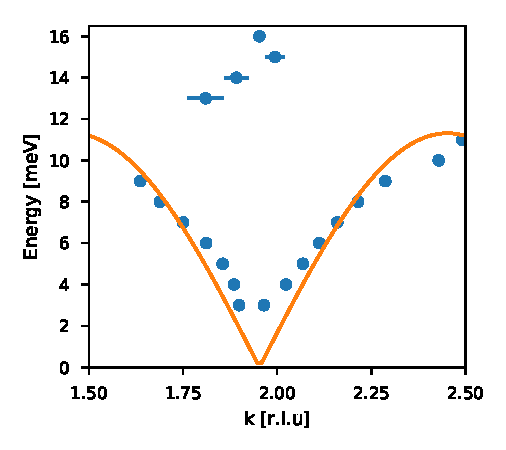
\includegraphics[width=0.45\textwidth]{fig/lowen/dispersion_220T.pdf}
    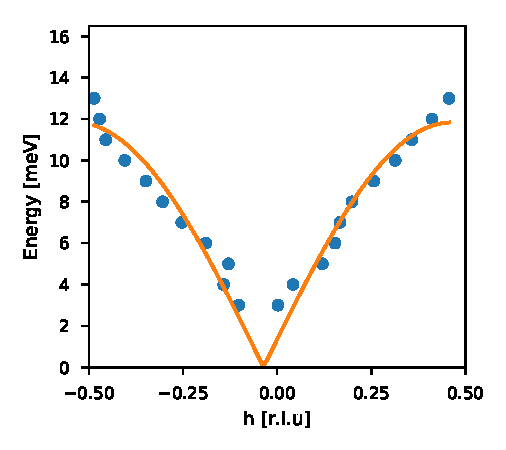
\includegraphics[width=0.45\textwidth]{fig/lowen/dispersion_400T.pdf}
    \caption[flatcone dispersion 220T/400T]{transverse flatcone dispersions at 220 (left) and 400 (right). Fit is a simple acoustic phonon dispersion for monoatomic systems: $\omega = \sqrt{4C/M} | \sin ( \pi (q-q_0) ) | $, where $M$ is the mass $C$ is the spring constant and $q_0$ is an offset to adjust for possible misalignment of the sample. $q$ is in reciprocal lattice units.}
    \label{fig:transverse_phonons_flatcone}
\end{figure}

\begin{figure}
    \centering
    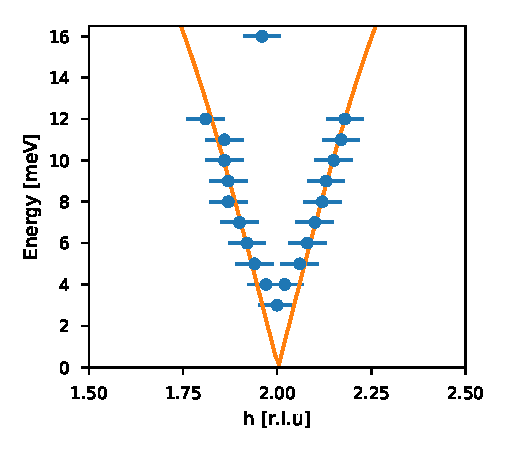
\includegraphics[width=0.45\textwidth]{fig/lowen/dispersion_220L.pdf}
    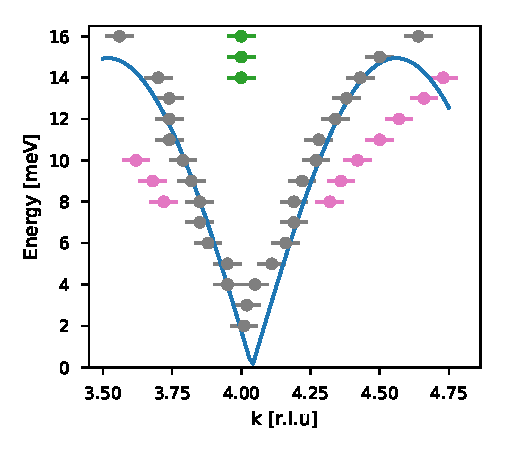
\includegraphics[width=0.45\textwidth]{fig/lowen/dispersion_400L.pdf}
    \caption[flatcone dispersion 220L/400L]{Longitudinal flatcone dispersions at 220 (left) and 400 (right). Fit is a simple acoustic phonon dispersion for monoatomic systems: $\omega = \sqrt{4C/M} | \sin ( \pi (q-q_0) ) | $, where $M$ is the mass $C$ is the spring constant and $q_0$ is an offset to adjust for possible misalignment of the sample. $q$ is in reciprocal lattice units.}
    \label{fig:longitudinal_phonons_flatcone}
\end{figure}

\begin{figure}
    \centering
    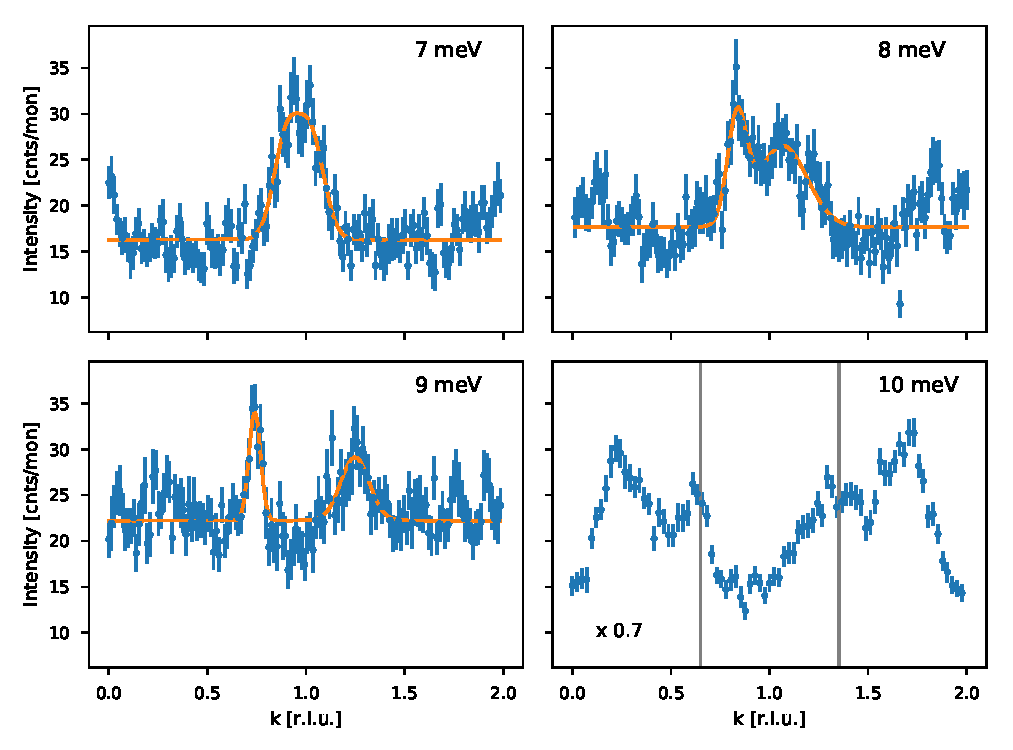
\includegraphics[width=0.8\textwidth]{fig/lowen/fits_310T.pdf}
    \caption[310T flatcone raw data]{310T flatcone raw data. The dispersion appears quite flat: $\delta_k = \{ 0.06, 0.12, 0.25, 0.35 \}$ for the 4 energies shown, with the last one (\SI{10}{\milli\eV}) being a very rough estimate from visual inspection. The direction is (400)-(220).}
    \label{fig:flatcone_phonons_310T_raw}    
\end{figure}

Figures \ref{fig:transverse_phonons_flatcone} and \ref{fig:longitudinal_phonons_flatcone} shows the peak positions as a function of energy along the transverse and longitudinal directions, respectively along with a naive fit to the shape of a monoatomic phonon dispersion \cite{Kittel2005}. Details about the peak finding feature and plots of the data is shown in appendix \ref{app:lowen_plots}. We have the expected results that longitudinal acoustic phonons are steeper since they are essentially bond stretching motions, where transverse phonons resembles a shear motion. Finally, we show the raw data for the four spectra where we see a signature of excitations around (310) in figure \ref{fig:flatcone_phonons_310T_raw}.

\begin{figure}
    \centering
    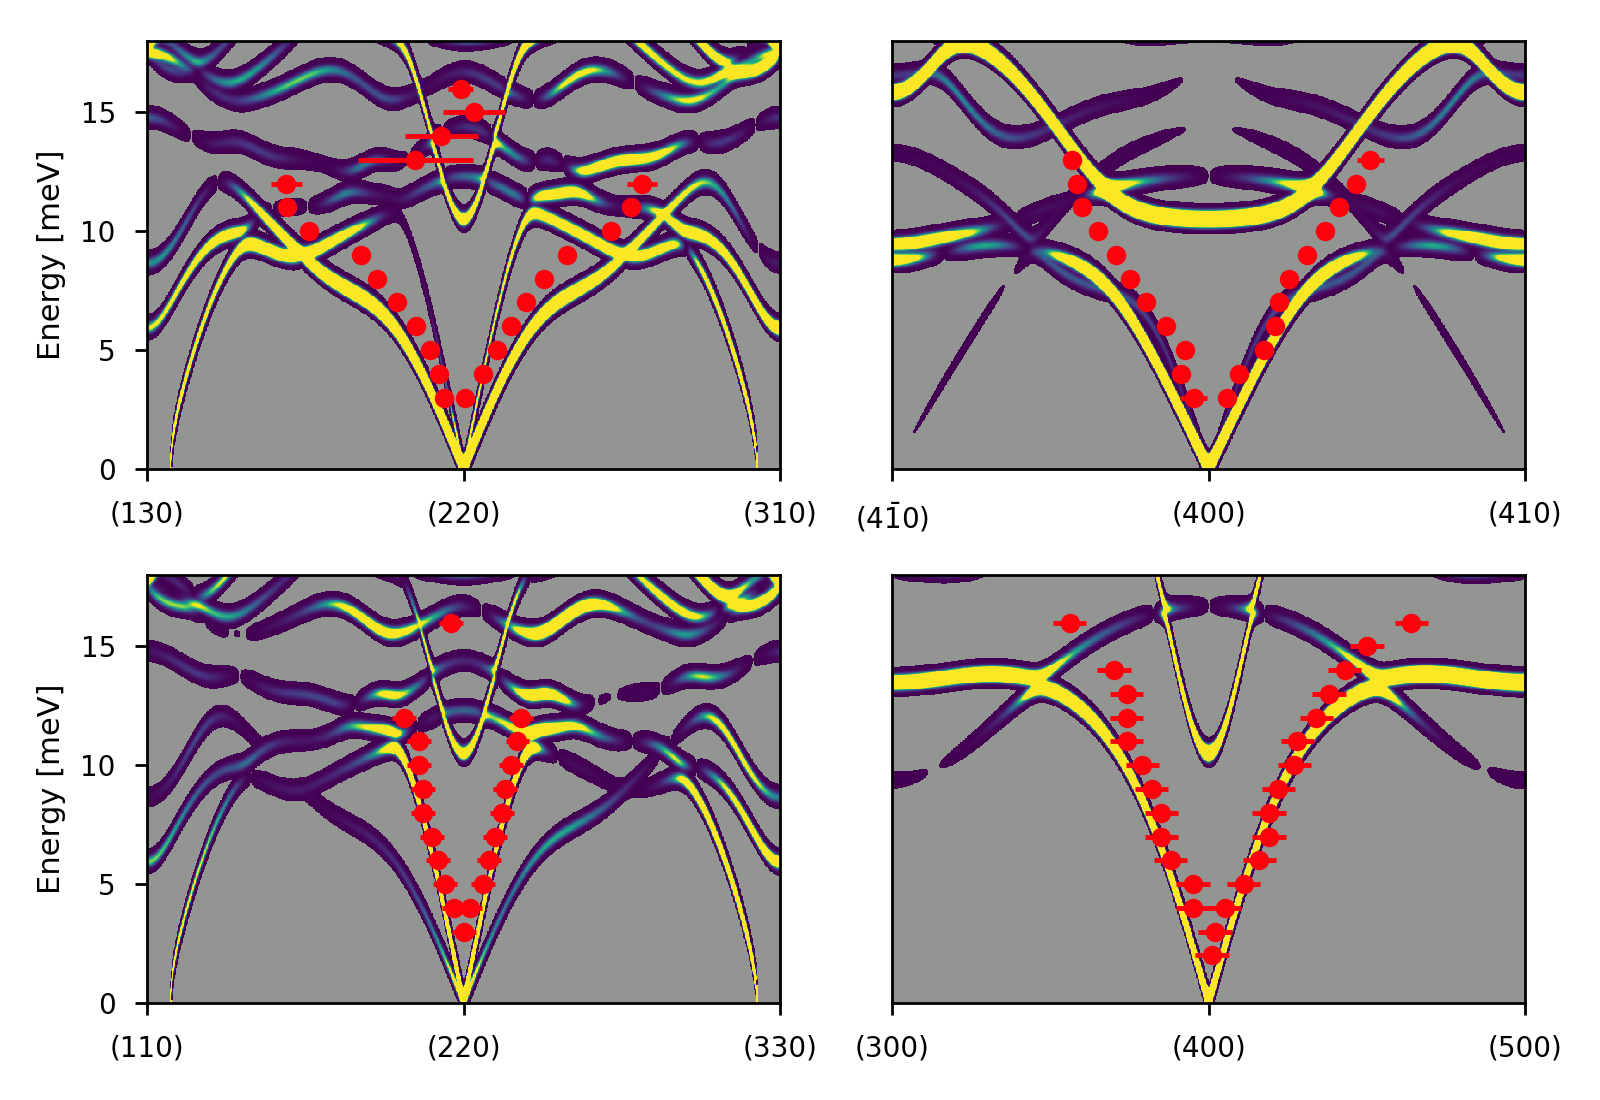
\includegraphics[width=\textwidth]{fig/lowen/flatcone_fits_simulation_lto_afm.png}
    \caption[FlatCone dispersion and neutron weighted simulation data]{Data obtained from FlatCone measurements in red (figures \ref{fig:transverse_phonons_flatcone} and \ref{fig:longitudinal_phonons_flatcone}) superimposed on the neutron-weighted simulation data of La$_2$CuO$_4$ in the orthorhombic phase. The simulation data is given a small Gaussian width in order to emphasize what a neutron experiment should look like according to simulations.}
    \label{fig:flatcone_phonons_dispersion_simulation}
\end{figure}

\begin{figure}
    \centering
    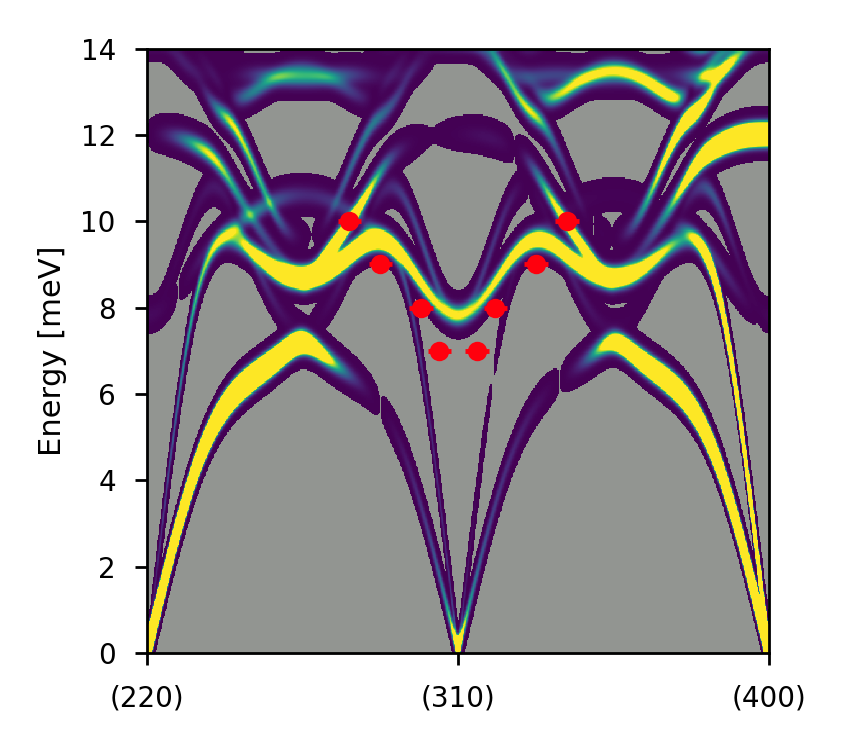
\includegraphics[width=0.5\textwidth]{fig/lowen/flatcone_fits_simulation_310T.png}
    \caption{FlatCone data of the shallow features observed in the transverse direction near (310) (figure \ref{fig:flatcone_phonons_310T_raw}), superimposed on neutron-weighted simulation data in the same direction.}
    \label{fig:flatcone_phonons_310T_sim}
\end{figure}

Once again, we can use this extracted dispersion to compare with our simulation data. In figure \ref{fig:flatcone_phonons_dispersion_simulation}, we see the data previous figures along with a neutron weighted band structure plot along the same directions. Once again, the simulations have been broadened along the energy axis in order to emphasize the neutron cross-section. This also means that there are certain bands not visible in these plots because their intensity vanishes (see figure \ref{fig:bands_sqw_color_line} for a visual explanation of this point). As indicated by the two dimensional color plot in figure \ref{fig:flatcone_raw_inelastic}, we have excellent agreement between measurement and simulation.

As the attentive reader might have noticed, we performed simulations of several different versions of La$_2$CuO$_4$ in chapter \ref{ch:simulation}. The comparison shown here is the low-temperature orthorhombic structural phase in the insulating state with static magnetism. This was chosen using through a visual inspection of the different simulations. The remaining five plots are shown in appendix \ref{app:lowen_plots}.

\begin{figure}
    \centering
    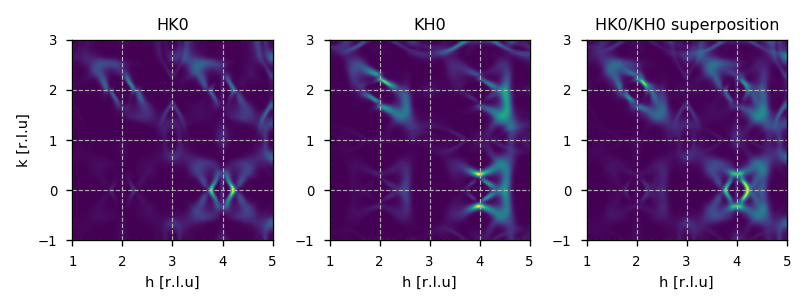
\includegraphics[width=\textwidth]{fig/lowen/simulation_colorplot_twin_comparison.png}
    \caption[Simulation comparison hkl khl]{Simulation data in the $a$-$b$ plane of La$_2$CuO$_4$ at 9 meV in the low-temperature orthorhombic phase. The first two images show the effect of exchanging the $a$ and $b$ directions when generating the plot and the last shows the superposition of the two.}
    \label{fig:lto_hk0_kh0_comparison}
\end{figure}

In addition, the bottom row of figure \ref{fig:flatcone_raw_inelastic} was generated taking twinning (see XX\todo{I should write about this early so i can refer back...}) into account. Since $a$ and $b$ directions in the low-temperature orthorhombic phase are close in length, twinning essentially makes the two directions indistinguishable. To show how this affects the dynamics, figure \ref{fig:lto_hk0_kh0_comparison} gives a visual indication of this superposition at \SI{9}{\milli\eV}. While the HK0/KH0 planes have a similar overall shape, it becomes clear that the superposition has the strongest resemblance to our data.

\begin{figure}
    \centering
    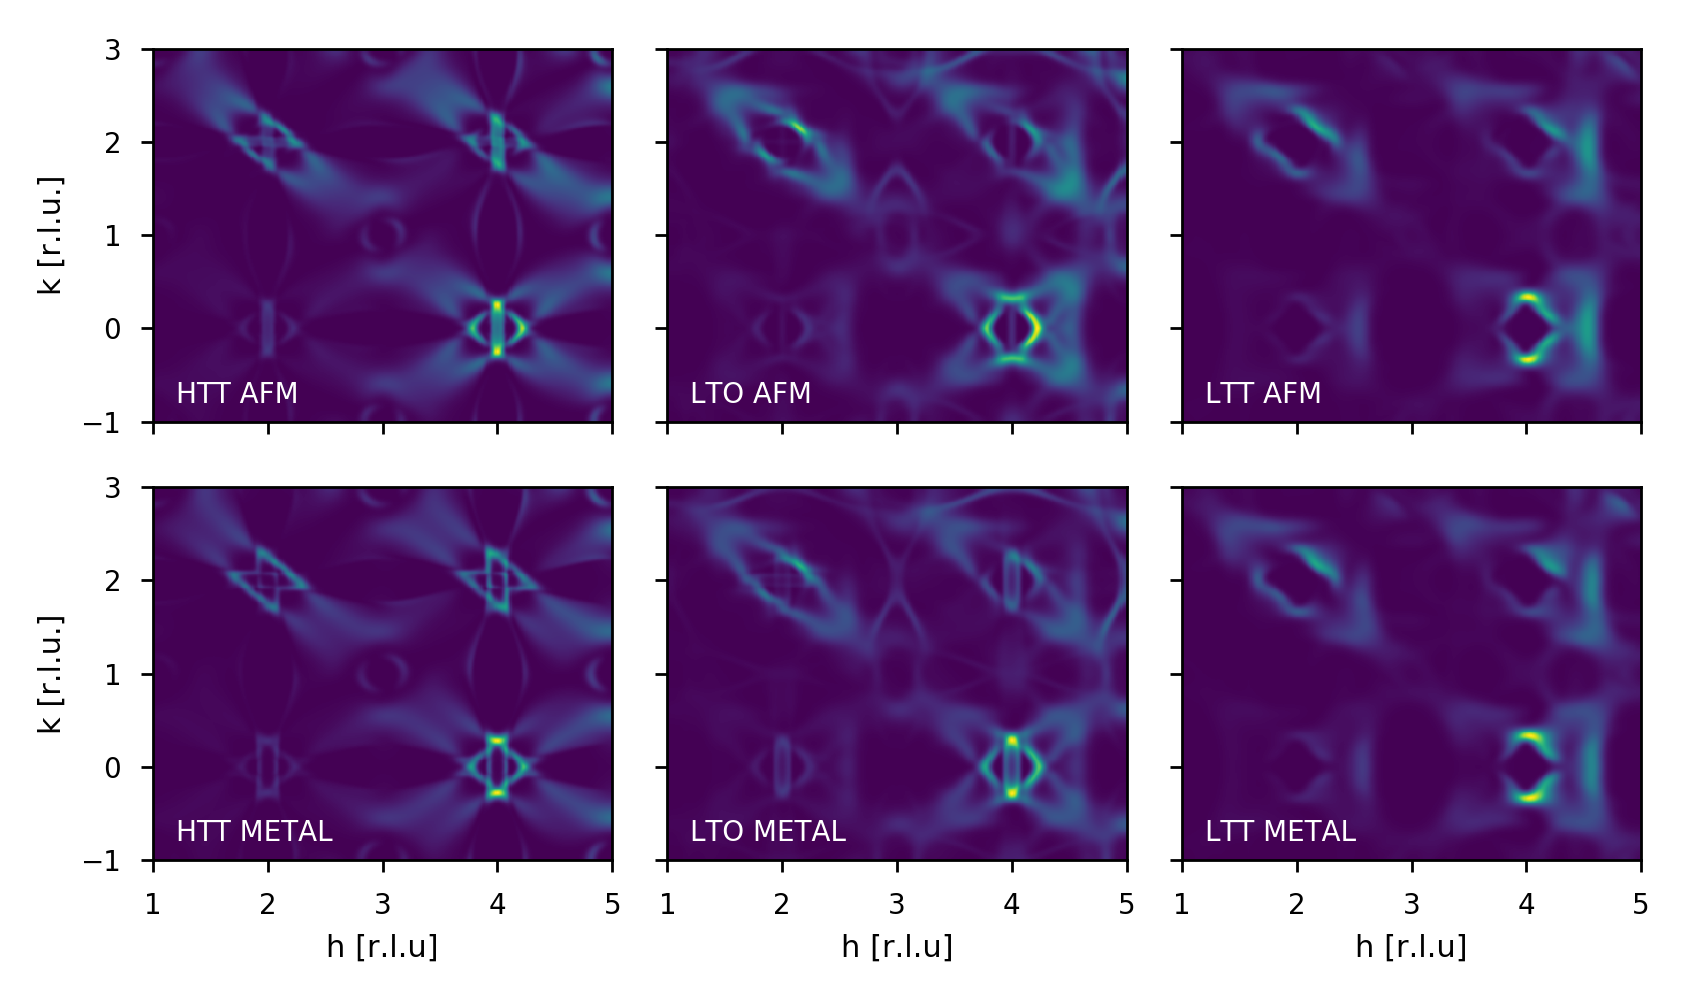
\includegraphics[width=\textwidth]{fig/lowen/twinning_plots_all.png}
    \caption[All qxqy plots at 9 meV including twinning for the LTO case]{Simulation data in the $a$-$b$ plane at \SI{9}{\milli\eV} from the six different phonon calculations performed in chapter \ref{ch:simulation}.}
    \label{fig:simulation_sqw_xy_plots_all}
\end{figure}

For the sake of completeness, figure \ref{fig:simulation_sqw_xy_plots_all} shows all six simulations from chapter \ref{ch:simulation} at \SI{9}{\milli\eV}. Once again, it seems likely that the `LTO AFM' simulation is the best representation of the sample chosen for this experiment, La$_{1.94}$Sr$_{0.06}$CuO$_{4+\delta}$.

While not groundbreaking in terms of scientific impact, I believe that these comparison confidently shows that our simulations can be trusted to some degree with regards to lattice dynamics. In addition, I hope that the tools (appendix \ref{app:software}) developed to generate these plots can be helpful for neutron scatterers in the future. To end this section, I direct the reader to a video at \url{https://youtu.be/LC-qV3CjqBM} which illustrates the dispersive features of the 2D colorplots in this section by moving through the energy axis as a function of time. While not particularly pertinent, I think it has an aesthetic most people can appreciate.

\section{Structural instabilities}
In this section, we investigate a peculiarity with regards to the low-temperature orthorhombic phase in La$_{2-x}$Sr$_x$CuO$_{4}$. In the mid 2000s, it was discovered that this material is unstable towards a low-temperature tetragonal phase at low temperatures. This shows up as the softening of a phonon at (104) and the temperature-dependence has been measured in optimally doped La$_{1.85}$Sr$_{0.15}$CuO$_4$ and insulating La$_{1.95}$Sr$_{0.05}$CuO$_4$, summarized in figure \ref{fig:soft_phonons_summary}. Back then, it was suggested that the softening abruptly stops at $T_\text{c}$ for the optimally doped sample, essentially preventing the tetragonal phase from emerging -- or at least stopping the instability in its tracks.

These ideas are consistent with the idea that lanthanum cuprates near $x=\frac{1}{8}$ have their $T_\text{c}$ suppressed due to the proximity of this tetragonal phase. This is particularly apparent in La$_{2-x}$Ba$_x$CuO$_4$ where the tetragonal phase appears and $T_\text{c}$ drops to a few Kelvin \cite{Hucker2012}.

\begin{figure}[]
    \centering
    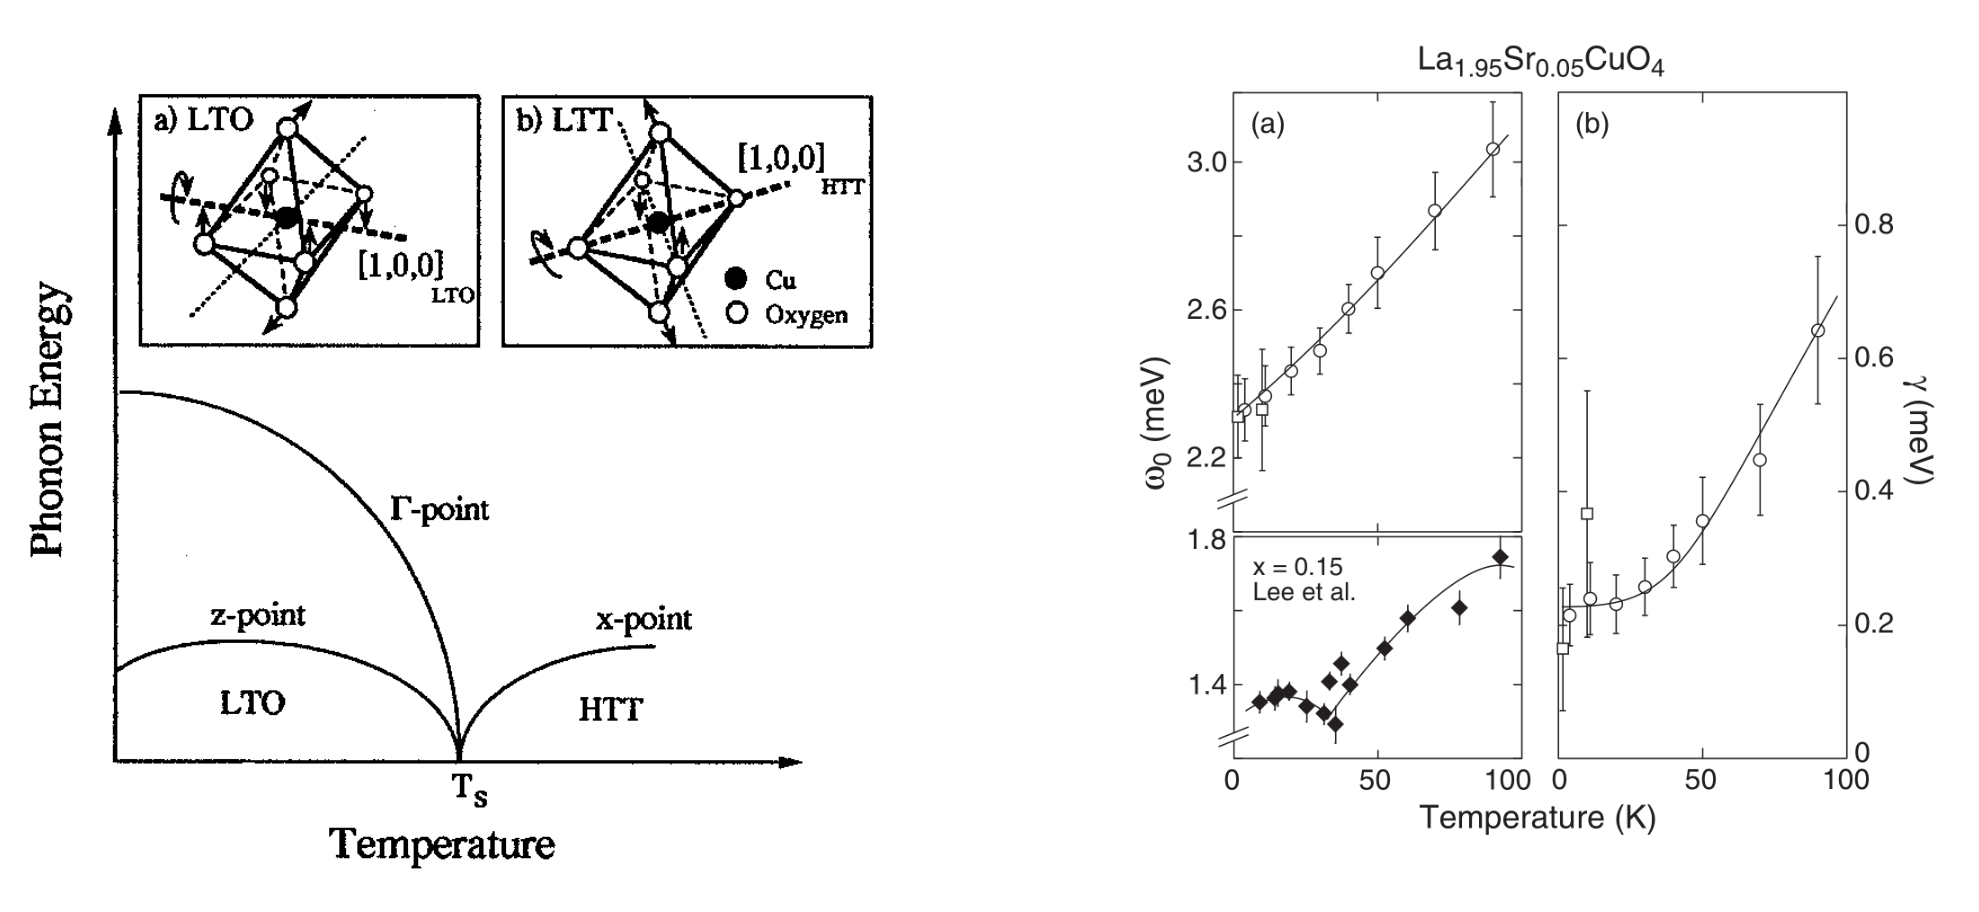
\includegraphics[width=\textwidth]{fig/lowen/soft_phonons.png}
    \caption{Soft phonons in La$_{2-x}$Sr$_x$CuO$_4$. \textbf{Right:} Schematic of the phonons related to structural phase transitions, with HTT being high-temperature tetragonal, LTO low-temperature orthorhombic and LTT low-temperature tetragonal. Decreasing the temperature across the structural phase transition temperature $T_\text{s}$, the $X$-point phonon becomes soft and finally splits into $\Gamma$ and $Z$-point phonon branches. \textbf{Right}: Measurements of the $Z$-point phonon in La$_{1.95}$Sr$_{0.05}$CuO$_4$ and La$_{1.85}$Sr$_{0.15}$CuO$_4$, showing a softening of this mode where the phonon energy $\omega_0$ decreases with decreasing temperature. This softening is associated with a sharpening of the linewidth $\gamma$.}
    \label{fig:soft_phonons_summary}
\end{figure}

We set out to do a similar experiment on the cold Triple-Axis ThALES at ILL. The sample is a single crystal La$_2$CuO$_{4+\delta}$ aligned in the $a$-$c$ plane. Measurements were constant-$\bm{Q}$ scans, and the temperature dependence is shown in figure \ref{fig:lcoo_zpoint_phonon_fits} and the summary of the fits are shown in \ref{fig:lcoo_zpoint_phonon_energies}.

\begin{figure}
    \centering
    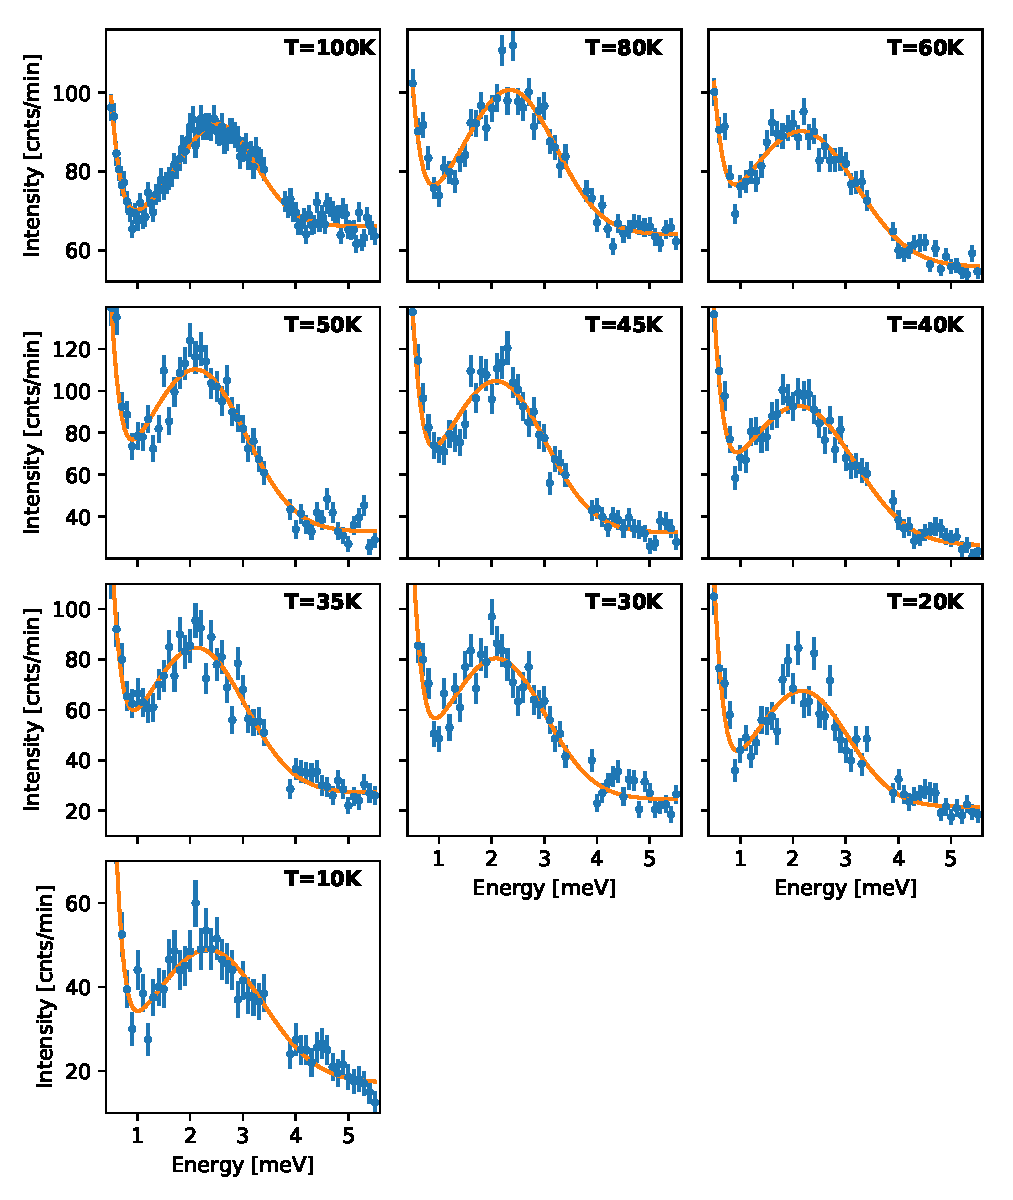
\includegraphics[width=\textwidth]{fig/lowen/lcoo_phonon_fits.pdf}
    \caption[lco+o Z-point phonon fits]{Measurements of the $Z$-point phonon in La$_2$CuO$_{4+\delta}$. At each temperature an energy scan from \SIrange{0.5}{5.5}{\milli\eV} is performed, clearly showing the phonon at $\approx \SI{2.5}{\milli\eV}$. The strong Bragg tail comes from the fact that we are measuring (104) and (014) simultaneously as a result of twinning. (104) is $Z$ in the orthorhombic phase, while (014) is $\Gamma$. The data is fitted to a sum of two Gaussian functions, describing the Bragg tail and phonon plus a constant background. The use of a Gasussian rather than Lorentzian for the phonon is phenological, since it described the data much better.}
    \label{fig:lcoo_zpoint_phonon_fits}
\end{figure}

\begin{figure}
    \centering
    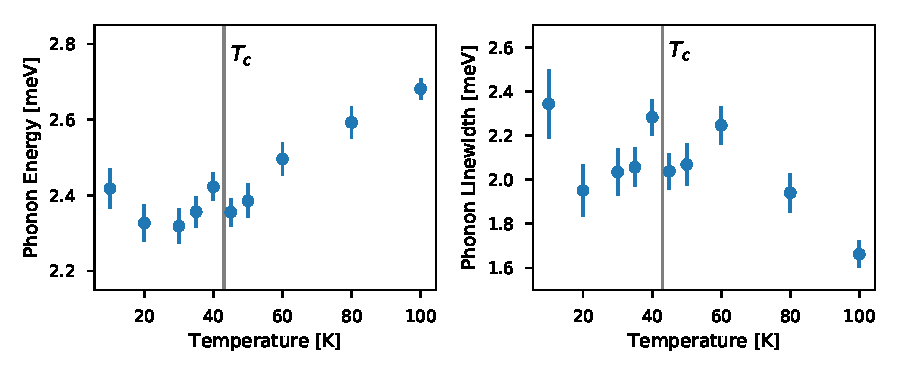
\includegraphics[width=\textwidth]{fig/lowen/lcoo_phonon_energies.pdf}
    \caption[lco+o Z-point phonon E-T plot]{Temperature dependence of the $Z$-point phonon in La$_2$CuO$_{4+\delta}$. \textbf{Left}: Phonon energy as a function of temperature. \textbf{Right:} Phonon linewidth as a function of temperatures, where the width corresponds to the Full-Width Half-Maximum of the Gaussian.}
    \label{fig:lcoo_zpoint_phonon_energies}
\end{figure}

We immediately notice that our experiment stands out when compared to LSCO5 and LSCO15. First, the energy dependence resembles that of LSCO15, but shifted up by \SI{1}{\milli\eV} and the linewidth has the opposite dependence of what one would expect and increases with decreasing temperature. In addition the linewidth is also increased by roughly \SI{1}{\milli\eV}. I stress here that we performed these experiments with an extremely tight energy resolution (roughly $\SI{0.1}{\milli\eV}$, see figure \ref{fig:phonon_resolution}), so the broadening is definitely unique to this system.

I foresee two scenarios causing this broadening. Either it is the expected broadening that is typically observed with soft phonons or it is caused by a splitting or distribution of modes at this energy. Three factors point to the second scenario. One, we know that the interstitial oxygen in La$_2$CuO$_{4+\delta}$ is spatially inhomogeneous, so it would not be surprising to have spatially separated regions with different `spring constants' for this phonon modes. In particular, we know that this mode is related to octahedral tilts which are affected by the interstitial near the apex of the CuO$_6$ octahedra. Second, the fitting procedure revealed that a Lorentzian function gives a poor description of the data as compared to a Gaussian. While not conclusive, this points to abnormal behavior which would be in favor of the second scenario. Third, we have the opposite temperature dependance of the linewidth when compared to La$_{1.95}$Sr$_{0.05}$CuO$_4$ and La$_{1.85}$Sr$_{0.15}$CuO$_4$ which, once again, points to these measurements being anomalous when compared to the strontium doped variants.

\begin{figure}
    \centering
    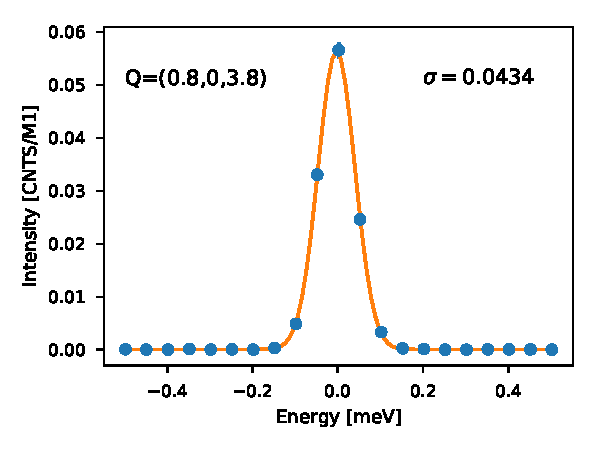
\includegraphics[width=0.5\textwidth]{fig/lowen/resolution_phonons.pdf}
    \caption{Energy resolution of ThALES in the conditions used to measure soft phonons. An energy scan at an arbitrary $\bm{Q} = (0.8,0,3,8)$ close to the (104) peak we are interested in reveals an energy resolution with a $\sigma = \SI{0.04}{\milli\eV}$ Gaussian with corresponding to \SI{0.10}{\milli\eV} Full-Width Half-Maximum.}
    \label{fig:phonon_resolution}
\end{figure}

\section{Low energy modes of superstructures}
Finally, we take a look at the superstructures observed in chapter \ref{ch:local} and use the Triple-Axis Spectrometer ThALES to look for a dynamic signature of these satellites. It is well known that structural peaks, per Goldstone's theorem, should have acoustic modes emerging from their position. 

\begin{figure}
    \centering
    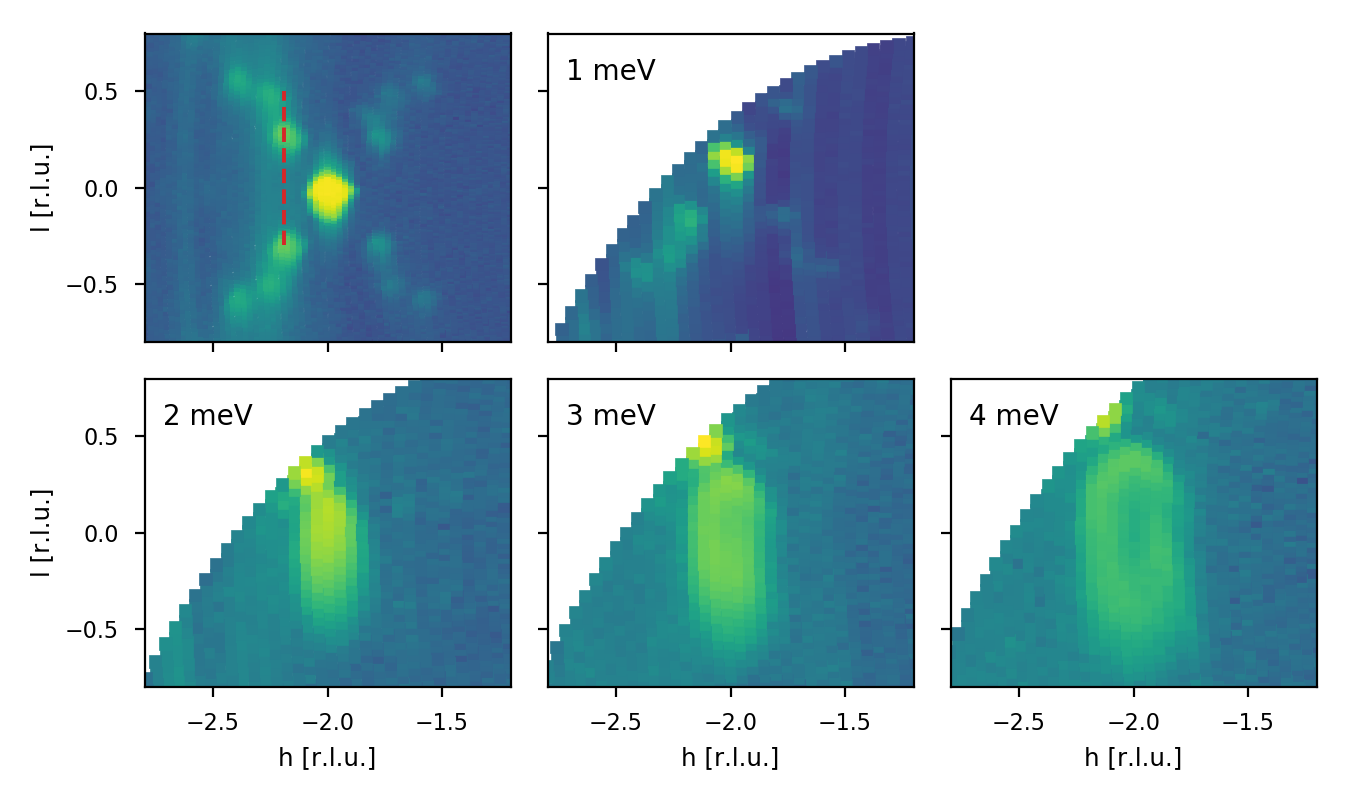
\includegraphics[width=\textwidth]{fig/lowen/phason_flatcone.png}
    \caption{FlatCone data of La$_2$CuO$_{4+\delta}$ in the $a$-$b$ plane in the elastic condition (top left) and at \SIlist{1;2;3;4}{\milli\eV} as indicated by the figures. In general, the energy-dependant features show no signature of superstructures, and we only see the acoustic phonon from the (200) Bragg peak.}
    \label{fig:phason_flatcone_maps}
\end{figure}

We start by looking at these dynamics with the FlatCone analyser as shown in figure \ref{fig:phason_flatcone_maps}. We, once again, clearly see the elastic scattering from the superstructures, but as we move up in energy, we only see the acoustic phonon emerging from the Bragg peak. Since the FlatCone analyser measures at a fixed energy, it can be difficult to see if the mode is very flat.

\begin{figure}
    \centering
    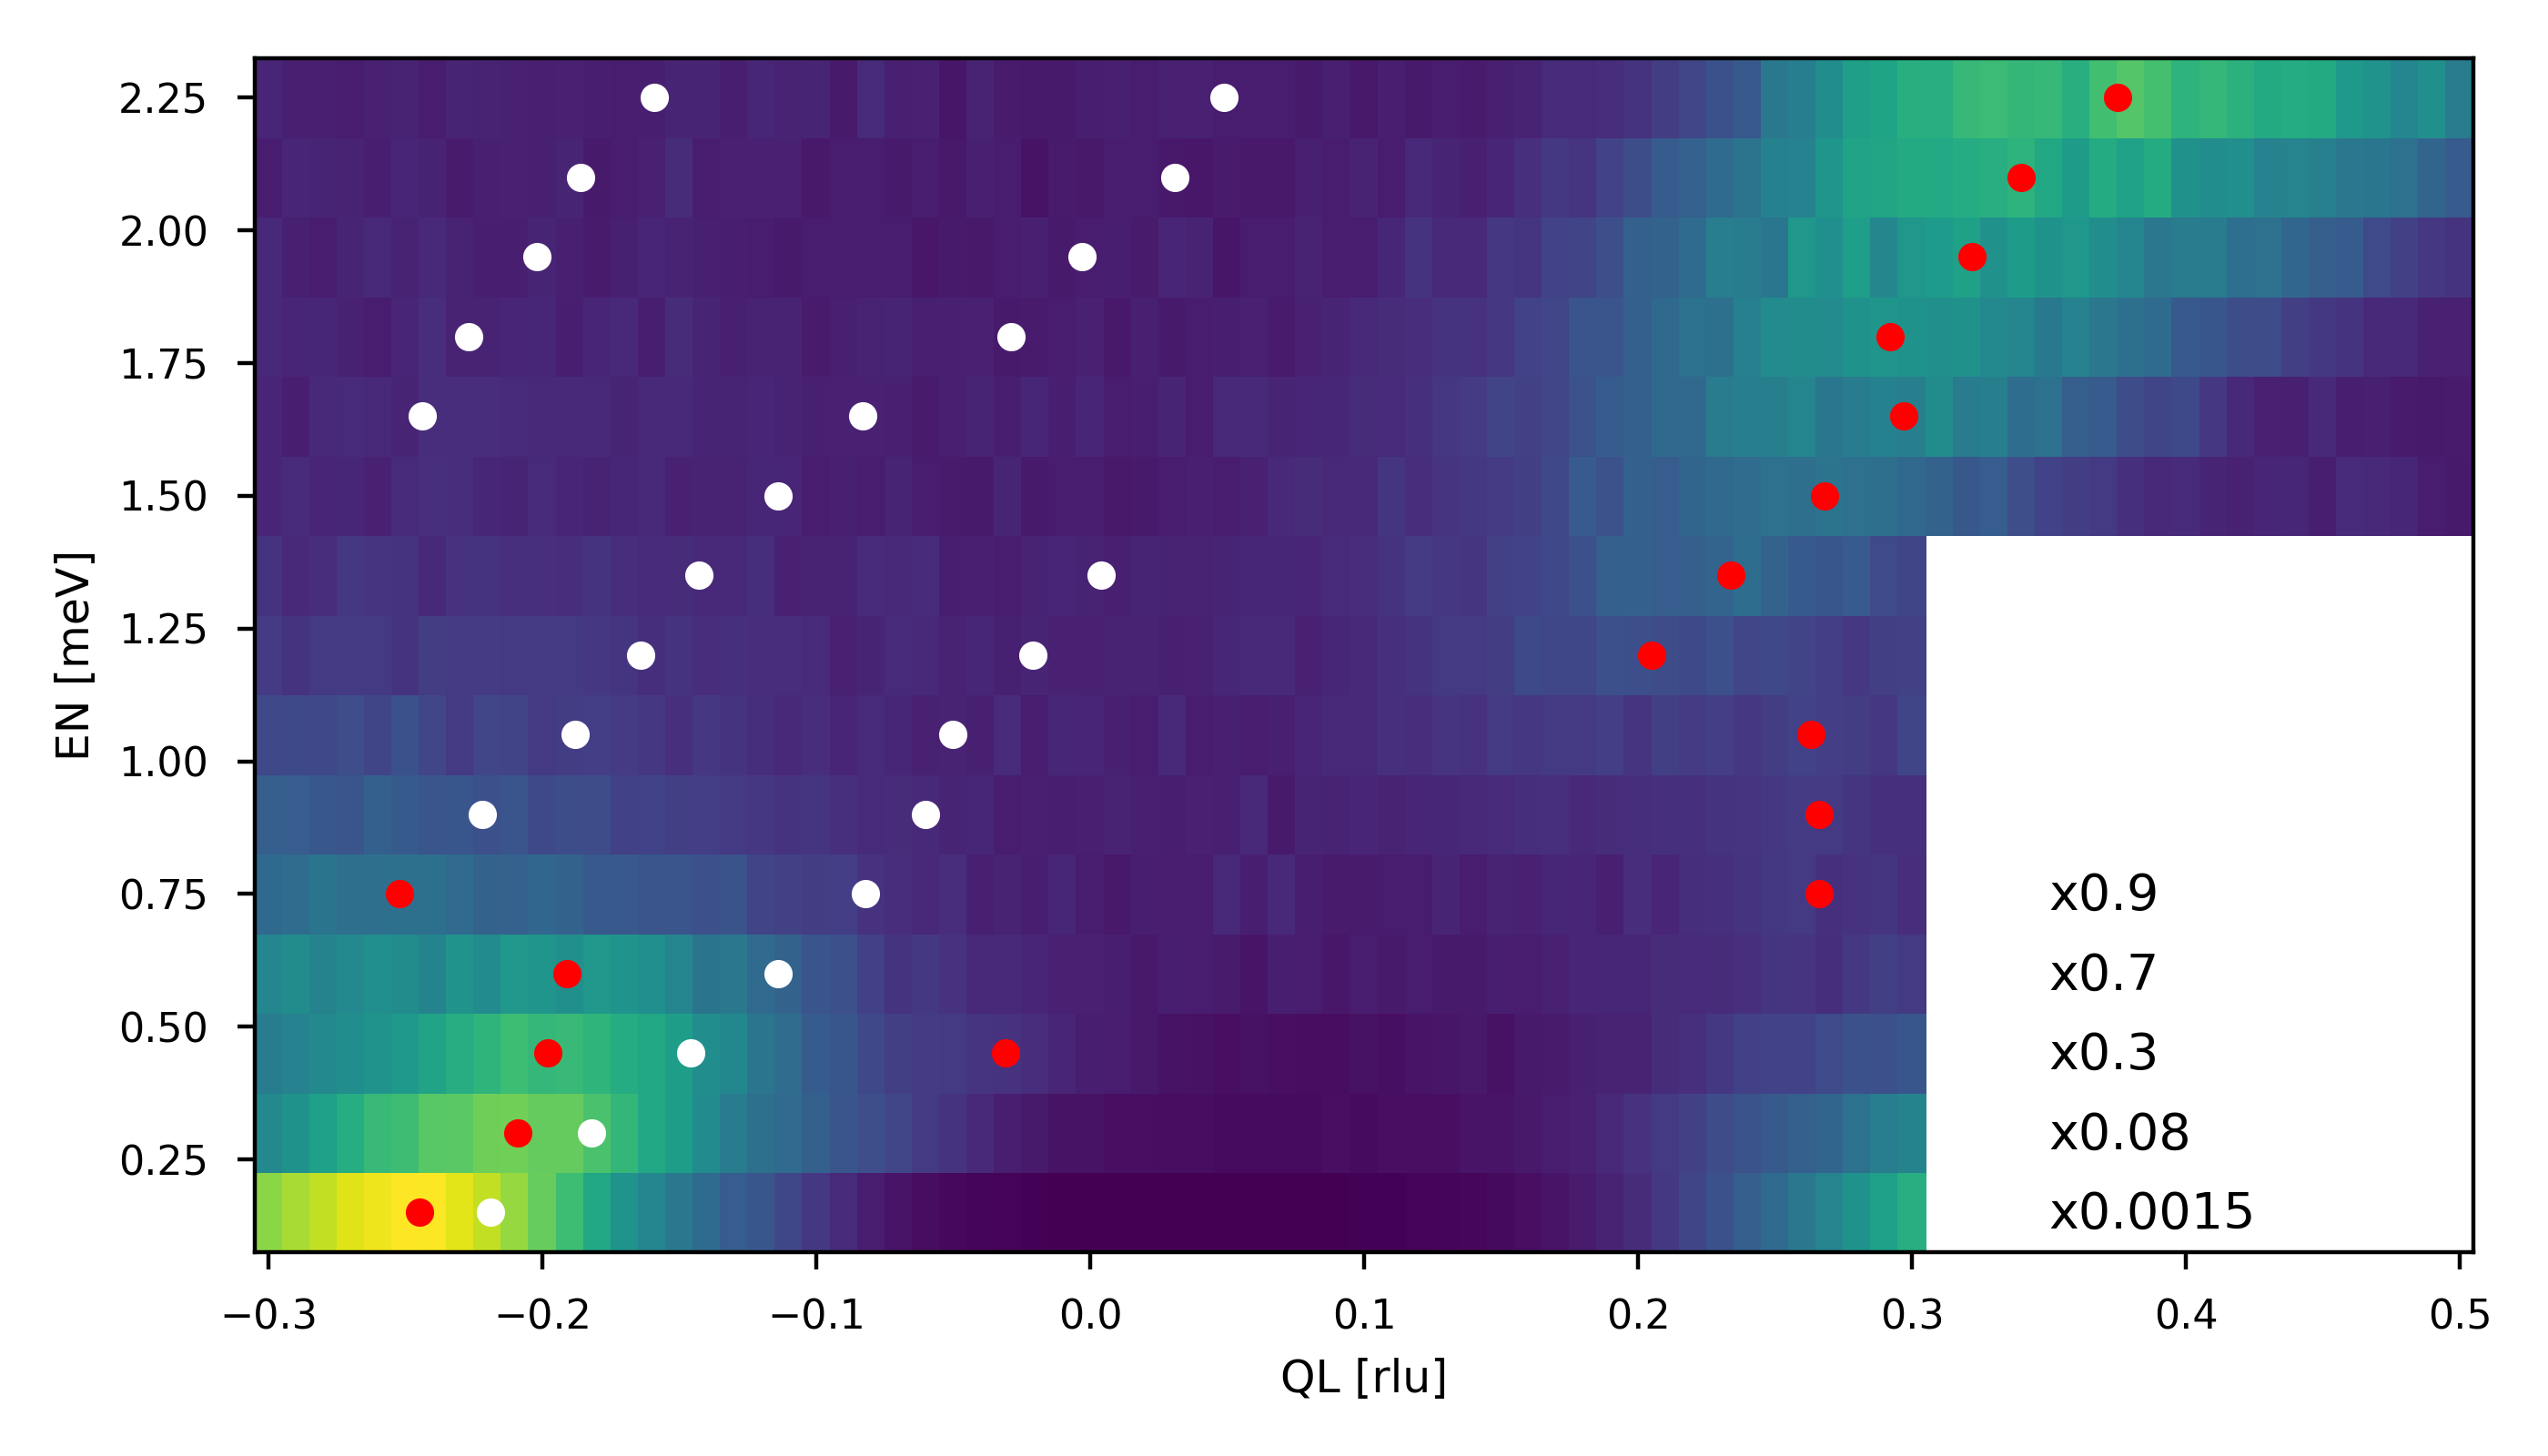
\includegraphics[width=0.85\textwidth]{fig/lowen/phason_colorplot.png}
    \caption[lack of phasons]{Data collected with a single-detector setup, designed to search for fundamental excitations from the satellite peaks as shown in figure \ref{fig:phason_flatcone_maps}, which also shows the direction where this data was obtained. The red and white markers indicate features visible in the individual scans, see appendix \ref{app:lowen_plots} for details. Due to the linear shape of these features, it seems likely that these are artifacts of the experiment.}
    \label{fig:lcoo_phasons_colorplot}
\end{figure}

For this reason, we switched to a single detector and made detailed measurements along the line shown in figure \ref{fig:phason_flatcone_maps}. The result is shown in figure \ref{fig:lcoo_phasons_colorplot}, revealing that we do not observe any phonon-like signature, despite very strong satellite reflections (roughly 20000 neutron counts per second). We even confirmed that we were in the best conditions possible with regards to resolution as shown in figure \ref{fig:phason_resolution}.

\begin{figure}
    \centering
    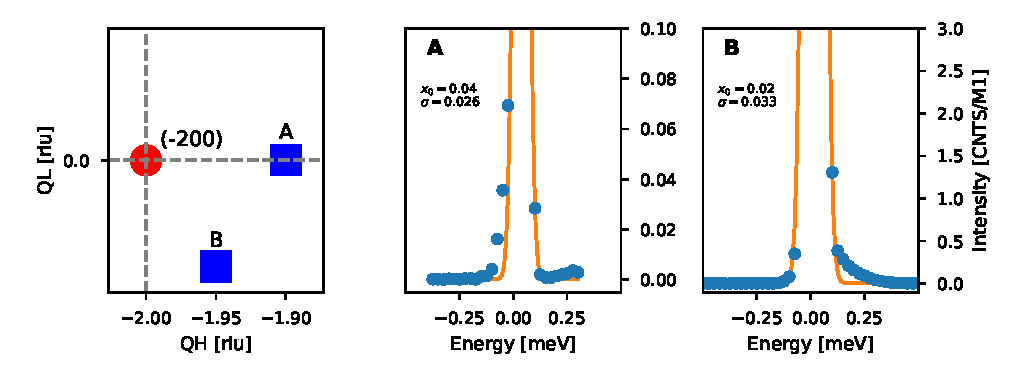
\includegraphics[width=\textwidth]{fig/lowen/resolution_phasons.pdf}
    \caption{Resolution in the experiment where we look for dynamics associated with superstructures. \textbf{Left}: Schematic of reciprocal space where we measured the energy-resolution of the instrument. I remark here that the superstructures are seen in the direction of \textbf{B}. Subfigures \textbf{A} and \textbf{B}, shows the raw data with a Gaussian fit at the two locations corresponding to the schematic. Since we are measuring close to the elastic Bragg peak, the increased intensity at \textbf{B} suggests that our resolution ellipsoid has points along the (200)-\textbf{B} direction.}
    \label{fig:phason_resolution}
\end{figure}

\section{Summary}
In this chapter, a few experiments concerning low-energy phonons were bundled together in order to help us better understand the dynamic nature of octahedral tilts in oxygen doped La$_2$CuO$_4$. We have shown that our simulations are highly reproducible in experiment, suggesting that we can expand our models to include interstitals through molecular dynamics in the next chapter. We also observed highly unusual behavior in La$_2$CuO$_{4+\delta}$ when trying to investigate soft phonons related to a structural instability. The behavior is significantly different from that of LSCO, but we still see a correlation between this phonon and $T_\text{c}$. Finally, we found no evidence of dynamics related to the well-known superstructures in La$_2$CuO$_{4+\delta}$, also highly unusual behavior.